%%%%%%%%%%%%%%%%%%%%%%%%%%%%%%%%%%%%%%%%%%%%%%%%%%%%%%%%%%%%%%%%%%%%%
% LaTeX Template: Project Titlepage Modified (v 0.1) by rcx
%
% Original Source: http://www.howtotex.com
% Date: February 2014
% 
% This is a title page template which be used for articles & reports.
% 
% This is the modified version of the original Latex template from
% aforementioned website.
% 
%%%%%%%%%%%%%%%%%%%%%%%%%%%%%%%%%%%%%%%%%%%%%%%%%%%%%%%%%%%%%%%%%%%%%%

\documentclass[12pt]{report}
\usepackage[utf8]{inputenc}
\usepackage[a4paper]{geometry}
\usepackage[myheadings]{fullpage}
\usepackage{fancyhdr}
\usepackage{lastpage}
\usepackage{graphicx, wrapfig, subcaption, setspace, booktabs}
\usepackage[T1]{fontenc}
\usepackage[font=small, labelfont=bf]{caption}
\usepackage{fourier}
\usepackage[protrusion=true, expansion=true]{microtype}
\usepackage[portuguese]{babel}
\usepackage{sectsty}
\usepackage{url, lipsum}
\usepackage{tgbonum}
\usepackage{hyperref}
\usepackage{xcolor}

\newcommand{\HRule}[1]{\rule{\linewidth}{#1}}
\onehalfspacing
\setcounter{tocdepth}{5}
\setcounter{secnumdepth}{5}


%-------------------------------------------------------------------------------
% TITLE PAGE
%-------------------------------------------------------------------------------

\begin{document}
{\fontfamily{cmr}\selectfont
\title{ \normalsize \textsc{}
		\\ [2.0cm]
		\HRule{0.5pt} \\
		\LARGE \textbf{\uppercase{Laboratório Sistemas Operacionais}
		\HRule{2pt} \\ [0.5cm]
		\normalsize \today \vspace*{5\baselineskip}}
		}

\date{}

\author{
		Gabriel Arcanjo Campelo Fadoul \\ 
		Universidade Federal de Roraima\\
		Departamento de Ciência da Computação}

\maketitle
\tableofcontents
\newpage

%-------------------------------------------------------------------------------
% Section title formatting
\sectionfont{\scshape}
\sectionmark
%-------------------------------------------------------------------------------

%-------------------------------------------------------------------------------
% BODY
%-------------------------------------------------------------------------------

\section{Introdução}
Este laboratório tem como intuito de colocar em prática todos os conhecimentos adquiridos durante as aulas de Sistemas Operacionais. Os softwares que serão utilizados serão:
\subsection{Sosim}
O Sosim, é um software educacional para apresentação simples e animada de como funciona um sistema operacional, principalmente os conceitos de gerência de processos e de memória virtual. Foi utilizada a versão 2.0 de 2007.

O SOsim foi desenvolvido pelo prof. Luiz Paulo Maia como parte de sua tese de mestrado no Núcleo de Computação Eletrônica da Universidade Federal do Rio de Janeiro (NCE/UFRJ), defendida em 2001 e orientada pelo prof. Ageu Pacheco. O objetivo deste trabalho foi desenvolver uma ferramenta gratuita que permitisse facilitar e melhorar as aulas de sistemas operacionais para alunos e professores.

\subsection{GCC 8.3.0}
Foi utilizado, para compilar todos os algoritmos referentes a este laboratório, o conjunto de compiladores GCC, mais especificamente, o G++ para compilar os arquivos que estão programados na linguagem C++. E também é importante ressaltar a utilização da biblioteca \textit{pthread} que deve ser adicionada ao compilar os programas.



\section{Questão 1 - Prática}
Essa seção se trata de atividades práticas se utilizando do software Sosim, que é um software educacional para apresentação simples e animada de como funciona um sistema operacional, principalmente os conceitos de gerência de processos e de memória virtual.

\subsection{Prática A}

A questão pergunta qual o motivo do software, quando criados dois processos, entrar em uma situação onde os dois processos estão no estado pronto, logo nenhum executando.

O motivo de existirem dois processos prontos para execução sé em razão do escalonamento. Quando um processo A termina sua execução, o escalonador verifica qual o próximo processo a ser executado. Isso causa um delay até que um outro proceso B, que foi escolhido pelo escalonador,seja executado.

\subsection{Prática B}
A pergunta trata dos motivos de ocorrer inanição (\textit{starvation}) durante a situação especificada pelo problema. Além de requisitar ações que um administrador de sistemas pode tomar para evitar esse tipo de situação.

De forma geral: Mesmo cada processo estando requisitando recursos diferentes, a forma de escalonamento faz com que o processo de maior prioridade sempre execute antes. Isso coloca o processo de menor prioridade em uma espera eterna, que é conhecido como uma situação de \textit{starvation}.

Uma ação que o administrador pode tomar é a utilizar uma estrutura para atribuir prioridades aos processos. A estrutura de fila funciona com a regra básica de que o primeiro elemento a entrar é o primeiro a sair. A utilização da mesma, evitaria a situação de inanição já que o processo sempre seria executado, independente de sua prioridade.

Outra ação, seria simplesmente igualar a prioridade dos processos. Com isso cada processo teria a mesma chance de ser escalonado, evitando assim o prolema de inanição.

\subsection{Prática C}
O problema trata sobre alocação de memória, e tem 3 perguntas relacionadas à esse tema:
\begin{enumerate}
    \item Qual o espaço de endereçamento real máximo de um processo?
    
    O espaço de endereçamento máximo é o tamanho da memória principal e o tamanho da memória secundária juntas.
    
    \item Qual o espaço de endereçamento real mínimo de um processo?
    
    O espaço de endereçamento mínimo é o tamanho mínimo da tabela de mapeamento de páginas.
    
    \item Qual o tamanho da página virtual?
    
    O tamanho é variável de acordo com a arquitetura do processador do computador.
\end{enumerate}
\newpage
\subsection{Prática D}

A questão também trata sobre memória virtual, mais especificamente  o funcionamento do algoritmo de paginação por demanda. Duas são as questões:
\begin{enumerate}
    \item Quais os critérios utilizados pelo simulador para selecionar o processo a ser transferido para o arquivo de paginação (swap out)?
    
    Os processos com menos chances de serem executados são armazenados na memória virtual.
    
    \item Quando o processo deve ser transferido novamente para a memória principal (swap in)?
    
    O processo somente retornará para a memória principal se ele certamente for executado pela CPU, ou seja, apenas quando for demandado.
\end{enumerate}

\section{Questão 2 - Banqueiro}
 O algoritmo do banqueiro é um algoritmo de escalonamento que tem como objetivo evitar impasses. Seu autor foi Dijkstra, e consiste no seguinte modelo: Um banqueiro de uma pequena cidade pode negociar com um grupo de clientes para os quais libera linha de crédito. O que o algoritmo faz é verificar se a liberação de uma requisição é capaz de levar a um estado inseguro(\textit{Deadlock}).Em caso positivo, a requisição será negada. Se a liberação de uma requisição levar a um estado seguro, ela será atendida. O primeiramente recebe do usuário a quantidade de processos e recursos disponíveis, e a partir daí ele gera uma matriz para representar esses processos, também é pedido ao usuário os recursos alocados e recursos máximos necessários de cada processo. Após isso, é executada uma varredura na matriz para verificar se algum processo já pode ser terminado, se sim, o processo é terminado e seus recursos recuperados, e a varredura reinicia. Caso não tenha processos para serem terminados, o programa informa que está em um estado inseguro e termina.
 
 Um exemplo de estado seguro é o da imagem abaixo:
 \begin{figure}[!ht]
	\centering
	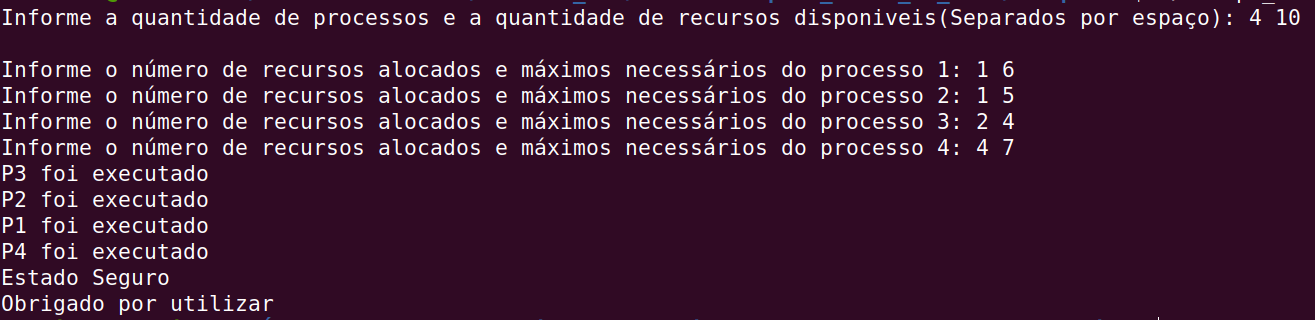
\includegraphics[width=0.8\textwidth]{BanqueiroSeguro.png}
	\caption{Saida Segura}
	\centering
	\label{label:file_name}
\end{figure}
Agora, um exemplo é este
\begin{figure}[!ht]
	\centering
	\includegraphics[width=0.8\textwidth]{BanqueiroIneguro.png}
	\caption{Saida Insegura}
	\centering
	\label{label:file_name}
\end{figure}

\section{Questão 3 - Barbeiro}
O problema do Barbeiro Dorminhoco é um problema clássico da ciência da computação, que trata de comunicação e sincronização de processos. O problema pode ser modelado da seguinte forma: Na barbearia há um barbeiro, uma cadeira de barbeiro e n cadeiras para eventuais clientes esperarem a vez. Quando não há clientes, o barbeiro senta-se na cadeira de barbeiro e cai no sono. Quando chega um cliente, ele precisa acordar o barbeiro. Se outros clientes chegarem enquanto o barbeiro estiver cortando o cabelo de um cliente, eles se sentarão (se houver cadeiras vazias) ou sairão da barbearia (se todas as cadeiras estiverem ocupadas). O problema é programar o barbeiro e os clientes sem cair em condições de disputa. Esse problema é semelhante a situações com várias filas, como uma mesa de atendimento de telemarketing com diversos atendentes e com um sistema computadorizado de chamadas em espera, atendendo a um número limitado de chamadas que chegam.

De forma geral, sua solução apresenta a utilização de threads e de semáforos para sincronizar a execução das mesmas. O intuito é fazer com que as threads fiquem executando indefinidamente, sem interrupções. O algoritmo desenvolvido não apresenta entrada de dados e sua saída desejada é a mostrada na imagem abaixo:

\begin{figure}[!ht]
	\centering
	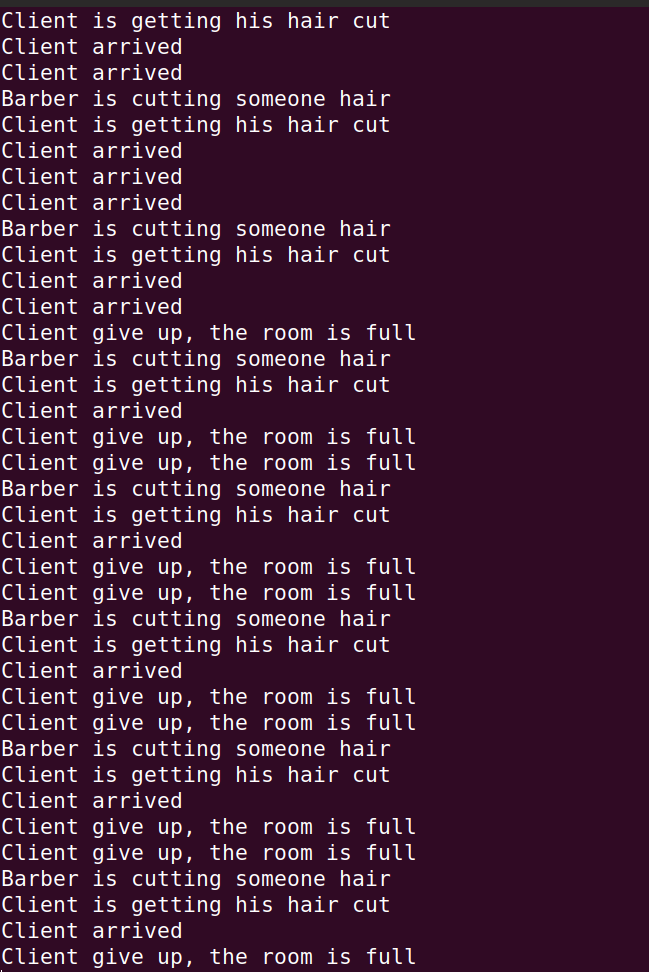
\includegraphics[width=0.8\textwidth]{Barbeiro.png}
	\caption{Saida desejada}
	\centering
	\label{label:file_name}
\end{figure}

}
\end{document}

%-------------------------------------------------------------------------------
% SNIPPETS
%-------------------------------------------------------------------------------

%\begin{figure}[!ht]
%	\centering
%	\includegraphics[width=0.8\textwidth]{file_name}
%	\caption{}
%	\centering
%	\label{label:file_name}
%\end{figure}

%\begin{figure}[!ht]
%	\centering
%	\includegraphics[width=0.8\textwidth]{graph}
%	\caption{Blood pressure ranges and associated level of hypertension (American Heart Association, 2013).}
%	\centering
%	\label{label:graph}
%\end{figure}

%\begin{wrapfigure}{r}{0.30\textwidth}
%	\vspace{-40pt}
%	\begin{center}
%		\includegraphics[width=0.29\textwidth]{file_name}
%	\end{center}
%	\vspace{-20pt}
%	\caption{}
%	\label{label:file_name}
%\end{wrapfigure}

%\begin{wrapfigure}{r}{0.45\textwidth}
%	\begin{center}
%		\includegraphics[width=0.29\textwidth]{manometer}
%	\end{center}
%	\caption{Aneroid sphygmomanometer with stethoscope (Medicalexpo, 2012).}
%	\label{label:manometer}
%\end{wrapfigure}

%\begin{table}[!ht]\footnotesize
%	\centering
%	\begin{tabular}{cccccc}
%	\toprule
%	\multicolumn{2}{c} {Pearson's correlation test} & \multicolumn{4}{c} {Independent t-test} \\
%	\midrule	
%	\multicolumn{2}{c} {Gender} & \multicolumn{2}{c} {Activity level} & \multicolumn{2}{c} {Gender} \\
%	\midrule
%	Males & Females & 1st level & 6th level & Males & Females \\
%	\midrule
%	\multicolumn{2}{c} {BMI vs. SP} & \multicolumn{2}{c} {Systolic pressure} & \multicolumn{2}{c} {Systolic Pressure} \\
%	\multicolumn{2}{c} {BMI vs. DP} & \multicolumn{2}{c} {Diastolic pressure} & \multicolumn{2}{c} {Diastolic pressure} \\
%	\multicolumn{2}{c} {BMI vs. MAP} & \multicolumn{2}{c} {MAP} & \multicolumn{2}{c} {MAP} \\
%	\multicolumn{2}{c} {W:H ratio vs. SP} & \multicolumn{2}{c} {BMI} & \multicolumn{2}{c} {BMI} \\
%	\multicolumn{2}{c} {W:H ratio vs. DP} & \multicolumn{2}{c} {W:H ratio} & \multicolumn{2}{c} {W:H ratio} \\
%	\multicolumn{2}{c} {W:H ratio vs. MAP} & \multicolumn{2}{c} {\% Body fat} & \multicolumn{2}{c} {\% Body fat} \\
%	\multicolumn{2}{c} {} & \multicolumn{2}{c} {Height} & \multicolumn{2}{c} {Height} \\
%	\multicolumn{2}{c} {} & \multicolumn{2}{c} {Weight} & \multicolumn{2}{c} {Weight} \\
%	\multicolumn{2}{c} {} & \multicolumn{2}{c} {Heart rate} & \multicolumn{2}{c} {Heart rate} \\
%	\bottomrule
%	\end{tabular}
%	\caption{Parameters that were analysed and related statistical test performed for current study. BMI - body mass index; SP - systolic pressure; DP - diastolic pressure; MAP - mean arterial pressure; W:H ratio - waist to hip ratio.}
%	\label{label:tests}
%\end{table}%\documentclass{article}
%\usepackage[utf8]{inputenc}

%\title{Weekly Report template}
%\author{gandhalijuvekar }
%\date{January 2019}

%\begin{document}

%\maketitle

%\section{Introduction}

%\end{document}
